\documentclass{beamer}

\usetheme{Singapore}

\usepackage{float}
\usepackage{multimedia}
\usepackage{color}
\usepackage{polski}
\usepackage[utf8]{inputenc}

\title{Wyrażenia regularne - regex}
\author{Ewa Namysł}
\institute{Uniwersytet Śląski}
\date{10 marca 2022}

\begin{document}

%STRONA TYTUŁOWA
\frame{
	\titlepage
}

%SPIS TREŚCI
\frame{
	\tableofcontents
	\frametitle{Spis treści}
}

%WSTĘP
\section{Czym są wyrażenia regularne?}
\frame{
	\frametitle{Czym są wyrażenia regularne?}
	\centering

	\textbf{Wyrażenia regularne}, w skrócie regex,\\
	to wzorce opisujące łańcuchy symboli.\\
	\vspace{1em}
	Upraszczając, jest to zbiór zasad opisujących\\
	jakiś tekst, zestaw znaków i cyfr etc.
}

\frame{
	\frametitle{Historia}
	\centering

	 W 1951 roku matematyk Stephen Cole Kleene stworzył podwaliny teorii opisującej języki regularne używając notacji matematycznej.\\
	\vspace{1em}
	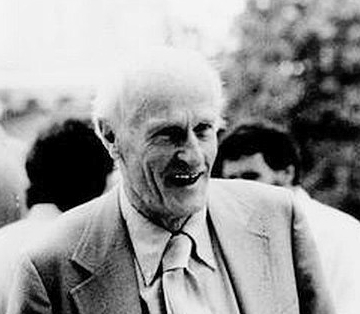
\includegraphics[scale=0.45]{kleene.jpg}
}

\frame{
	\centering

	Regex zyskał na popularności pod koniec lat sześćdziesiątych wraz z rozwojem Unixa.\\
	\vspace{2em}
	Ken Thompson, współtwórca Unixa, jako jeden z pierwszych wykorzystał notację Kleene'a w edytorze tekstu \textit{QED}.\\
	\vspace{0.5em}
	Thompson stworzył również na własny użytek narzędzie wyszukujące pliki według wzorców regexa.\\
	Obecnie znamy to narzędzie pod nazwą \textit{grep}.
	\vspace{2em}
	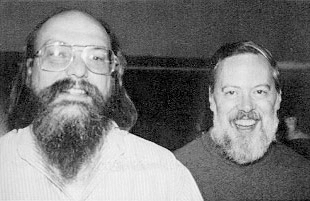
\includegraphics[scale=0.45]{thompson_ritchie.jpg}
}

\frame{
	\frametitle{Co zyskujemy?}
	\centering
	
	Dzięki wyrażeniom regularnym jesteśmy w stanie odnaleźć w tekście wszystkie wystąpienia danego wzorca.\\
	\vspace{1em}
	Jeśli poszukujemy konkretnego słowa, odnajdziemy je jako osobny string, ale również jeśli występuje jako składowa część wyrazu.
}

\frame{
	\frametitle{Przykład}
	\centering

	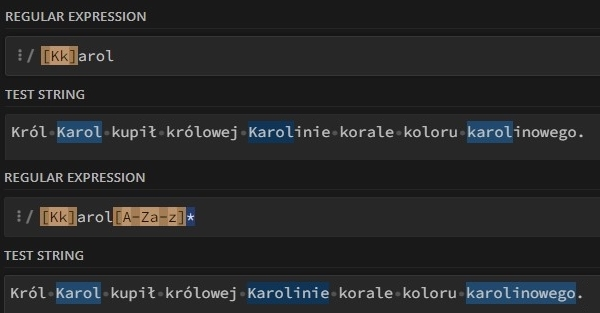
\includegraphics[scale=0.5]{przyklad1.jpg}
}


\frame{
	\frametitle{Popularne zastosowania}

	\begin{itemize}
		\item Walidacja danych - sprawdzanie adresów mailowych, kodów pocztowych etc.
		\item Webscraping - zautomatyzowane pozyskiwanie danych ze stron internetowych.
		\item Modyfikacja i podmienianie łańcuchów znaków, obróbka danych.
		\item Edytory tekstu, kompilatory.
	\end{itemize}
	\vspace{1em}
	Wiele programów i komend Linuxa wykorzystuje regexy, m.in.\\
	\textit{grep}, \textit{sed}, \textit{find}.\\
	\vspace{1em}
	Większość współczesnych języków programowania ma własne biblioteki obsługujące regexy, np. \textit{re} w Pythonie.
}

%SKŁADNIA
\section{Składnia}
\frame{
	\frametitle{Składnia}
	\centering

}

%PRZYKŁADY W PRAKTYCE
\section{Przykłady w praktyce}
\frame{
	\frametitle{Praktyczne przykłady}
	\centering

}

%PODSUMOWANIE
\section{Podsumowanie}
\frame{
	\frametitle{Podsumowanie}
	\centering

}

\frame{
	\frametitle{Bibliografia:}
	%zmienić!
	K. Beck, \emph{Extreme Programming Explained: Embrace Change}, Addison-Wesley, 2018.\\
	\vspace{1em}
	D. Wells, \emph{Extreme Programming},  http://www.extremeprogramming.org (dostęp marzec 2022).\\
	\vspace{1em}
	A. Kolm, \emph{Zarządzanie projektami IT}, http://zarzadzanieprojektami.it/ (dostep marzec 2022).\\
}

\end{document}